% title: 정적분과 넓이
% description: 곡선 y = f(x) 아래, x = a부터 x = b까지의 넓이(정적분)를 색칠한다. a, b 표시와 적분 기호
% packages: pgfplots
% libraries:
% f와 적분 구간 a, b만 바꾼다. 색칠은 \closedcycle이 곡선을 x축(y = 0)까지 닫아서 만든다.
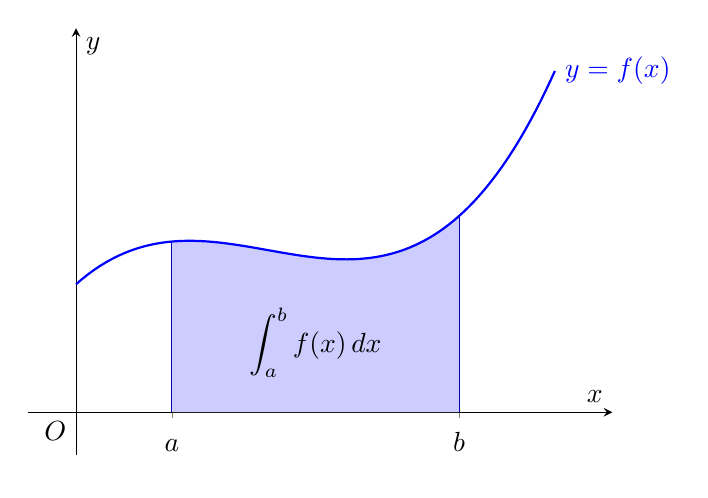
\begin{tikzpicture}[declare function={
    f(\x) = 0.1*\x^3 - 0.6*\x^2 + \x + 1.5;
  }]
  \def\a{1}
  \def\b{4}
  \begin{axis}[
      width=9cm, height=7cm,
      axis lines=middle, xmin=-0.5, xmax=5.6, ymin=-0.5, ymax=4.5,
      xlabel={$x$}, ylabel={$y$}, xtick={\a,\b}, xticklabels={$a$,$b$}, ytick=\empty,
      typeset ticklabels with strut,
      samples=100, clip=false]
    \addplot[fill=blue!20, draw=none, domain=\a:\b] {f(x)} \closedcycle;
    \draw[blue!70!black] (\a,0) -- (\a,{f(\a)});
    \draw[blue!70!black] (\b,0) -- (\b,{f(\b)});
    \addplot[thick, blue, domain=0:5] {f(x)} node[right] {$y=f(x)$};
    \node at ({(\a+\b)/2}, {0.45*f((\a+\b)/2)}) {$\displaystyle\int_a^b f(x)\,dx$};
    \node[below left] at (0,0) {$O$};
  \end{axis}
\end{tikzpicture}
